\documentclass[11pt]{article}
\usepackage[T1]{fontenc}
\usepackage[utf8]{inputenc}
\usepackage{amsmath,amssymb,amsthm}
\usepackage{mathtools}
\usepackage[numbers]{natbib}
\usepackage{graphicx}
\usepackage{hyperref}
\usepackage{cleveref}
\usepackage{microtype}

% TODO: Adjust metadata once author list and title are finalized.
\title{Adaptive Resistance Principle for Navier--Stokes}
\author{Author List}
\date{\today}

\begin{document}

\maketitle

\begin{abstract}
We present a control-theoretic viewpoint on the three-dimensional incompressible Navier--Stokes equations through the \emph{Adaptive Resistance Principle} (ARP), an adaptive law originally developed to stabilize complex dynamical systems.
The Clay Millennium problem asks whether smooth, globally-defined solutions exist for all smooth divergence-free initial data and body forces.
Our contribution is twofold: (i) an \emph{analytical lens} where an auxiliary ARP state $G(t)\ge 0$ driven by an intensity functional $\Phi(u)$ augments the classical energy method, yielding a Lyapunov-like quantity $V(t)=E(t)+\lambda G(t)$ with tunable dissipation; and (ii) a \emph{numerical framework} in which ARP-inspired adaptation stabilizes GPU-accelerated vorticity-based solvers at high Reynolds numbers.
This manuscript does not claim a resolution to the Millennium problem; instead, it proposes a tractable route for deriving a priori bounds and reports preliminary computational behavior consistent with enhanced stability.
\end{abstract}

\tableofcontents
\clearpage

\section{Introduction}
Despite a century of advances, global existence and smoothness for 3D incompressible Navier--Stokes remain open \citep{fefferman2006ns,clayproblem}.
We introduce a complementary \emph{Adaptive Resistance Principle} (ARP) lens: with an auxiliary $G$ driven by $\Phi(u)$, set $V=E+\lambda G$ to tune dissipation analytically and to guide adaptive stabilization numerically.

\section{Notation and setting}
$\Omega=\mathbb{T}^3$ (periodic, mean-zero). $E=\tfrac12\norm{u}_2^2$, $\Omega(t)=\norm{\omega}_2^2$. Poincar\'e: $\norm{u}_2^2\le C_P \norm{\nabla u}_2^2$.

\section{Preliminaries}
Navier--Stokes: $\partial_t u+(u\cdot\nabla)u+\nabla p=\nu\Delta u + f$, $\divergence u=0$, $\omega=\curl u$.
Energy: $\dot E=-\nu\norm{\nabla u}_2^2+\langle u,f\rangle$.

\section{ARP-augmented framework}
Choose $\Phi=\norm{\omega}_2^2$ and $V=E+\lambda G$ with $\dot G=\alpha \Phi - \mu G$.
Then $\dot V=-(\nu-\lambda\alpha)\norm{\omega}_2^2 + \langle u,f\rangle - \lambda\mu G$; for $f\equiv0$ and $\lambda\alpha<\nu$ this gives strict enstrophy dissipation.

\section{Main Theorem (Target B)}\label{sec:main_theorem}
Let $u_0\in H^m(\mathbb{T}^3)$, $m\ge 3$, $f\equiv0$.
Drive $G_k$ by $\dot G_k=\alpha_k\norm{\nabla^k\omega}_2^2-\mu_k G_k$ and set $V_m=\sum_{j=0}^{m-1}(E_j+\lambda_j G_j)$.
If for some $c_j>0$, $C_m\ge0$,
$\dot V_m \le -\sum_{j=0}^{m-1} c_j \norm{\nabla^{j+1}u}_2^2 + C_m$,
then the classical solution extends globally and remains smooth.

\section{Key lemmas}
\begin{lemma}[H$^1$ balance with ARP share]
$\frac{\dd}{\dd t}(E_0+E_1+\lambda_0 G_0+\lambda_1 G_1)
\le -\tfrac12(\nu-\lambda_1\alpha_1)\norm{\nabla\omega}_2^2 - \lambda_0\mu_0 G_0 - \lambda_1\mu_1 G_1 + C \Omega^{3/2}$.
\end{lemma}
\begin{lemma}[H$^m$ balance with commutators]
Assuming $| \int \nabla^k((\omega\cdot\nabla)u)\cdot \nabla^k\omega| \le \varepsilon_k \norm{\nabla^{k+1}\omega}_2^2 + C_k \Xi_k$, with $\varepsilon_k=\tfrac12(\nu-\lambda_k\alpha_k)$, then $\dot V_m \le -\sum_{j=0}^{m-1}\tfrac12(\nu-\lambda_j\alpha_j)\norm{\nabla^{j+1}u}_2^2 - \sum_j \lambda_j\mu_j G_j + C_m$.
\end{lemma}

\section{Proof program and gaps}
\textbf{Step 1:} Base level with $\lambda_0\alpha_0<\nu$ gives decay. 
\textbf{Step 2:} $H^1$ level; control vortex-stretching by $\varepsilon\|\nabla\omega\|_2^2+C_\varepsilon\Omega^{3/2}$ (Gap A).
\textbf{Step 3:} $H^m$ levels; commute and use $\varepsilon\|\nabla^{k+1}\omega\|_2^2+C_\varepsilon\Xi_k$ (Gap B).
\textbf{Step 4:} Sum and absorb via the schedule, yielding the master inequality.
\subsection*{Constant bookkeeping and $\varepsilon$ policy}
Let $\lambda_k\alpha_k\le \eta\nu$ with $\eta\in(0,1/4)$; pick $\varepsilon_k=\tfrac12(\nu-\lambda_k\alpha_k)$ to absorb high-derivative dissipation at each level.

\section{Numerical details}
3D vorticity-form solver (periodic) with spectral derivatives; semi-implicit viscosity, explicit nonlinearity; ARP-inspired time-step controller $\Delta t^{n+1}=\min\{\Delta t_{\max},(c_0+c_1 G^{n+1})/(1+c_2\Phi^n)\}$ and mild high-$k$ filters.

\section{ARP cascade parameter schedule}\label{sec:param_schedule}
For $k=0,\dots,m-1$, set $\alpha_k=a\,2^{-k}$, $\lambda_k=\ell\,2^{-k}$, $\mu_k=\mu_0$ with $a,\ell,\mu_0>0$.
Require $\lambda_k\alpha_k=a\ell\,2^{-2k} \le \eta \nu$ for all $k$; we target $\eta=\tfrac14$ so $(\nu-\lambda_k\alpha_k)\ge \tfrac34 \nu$.

\section{Preliminary results (placeholders)}
\begin{figure}[t]\centering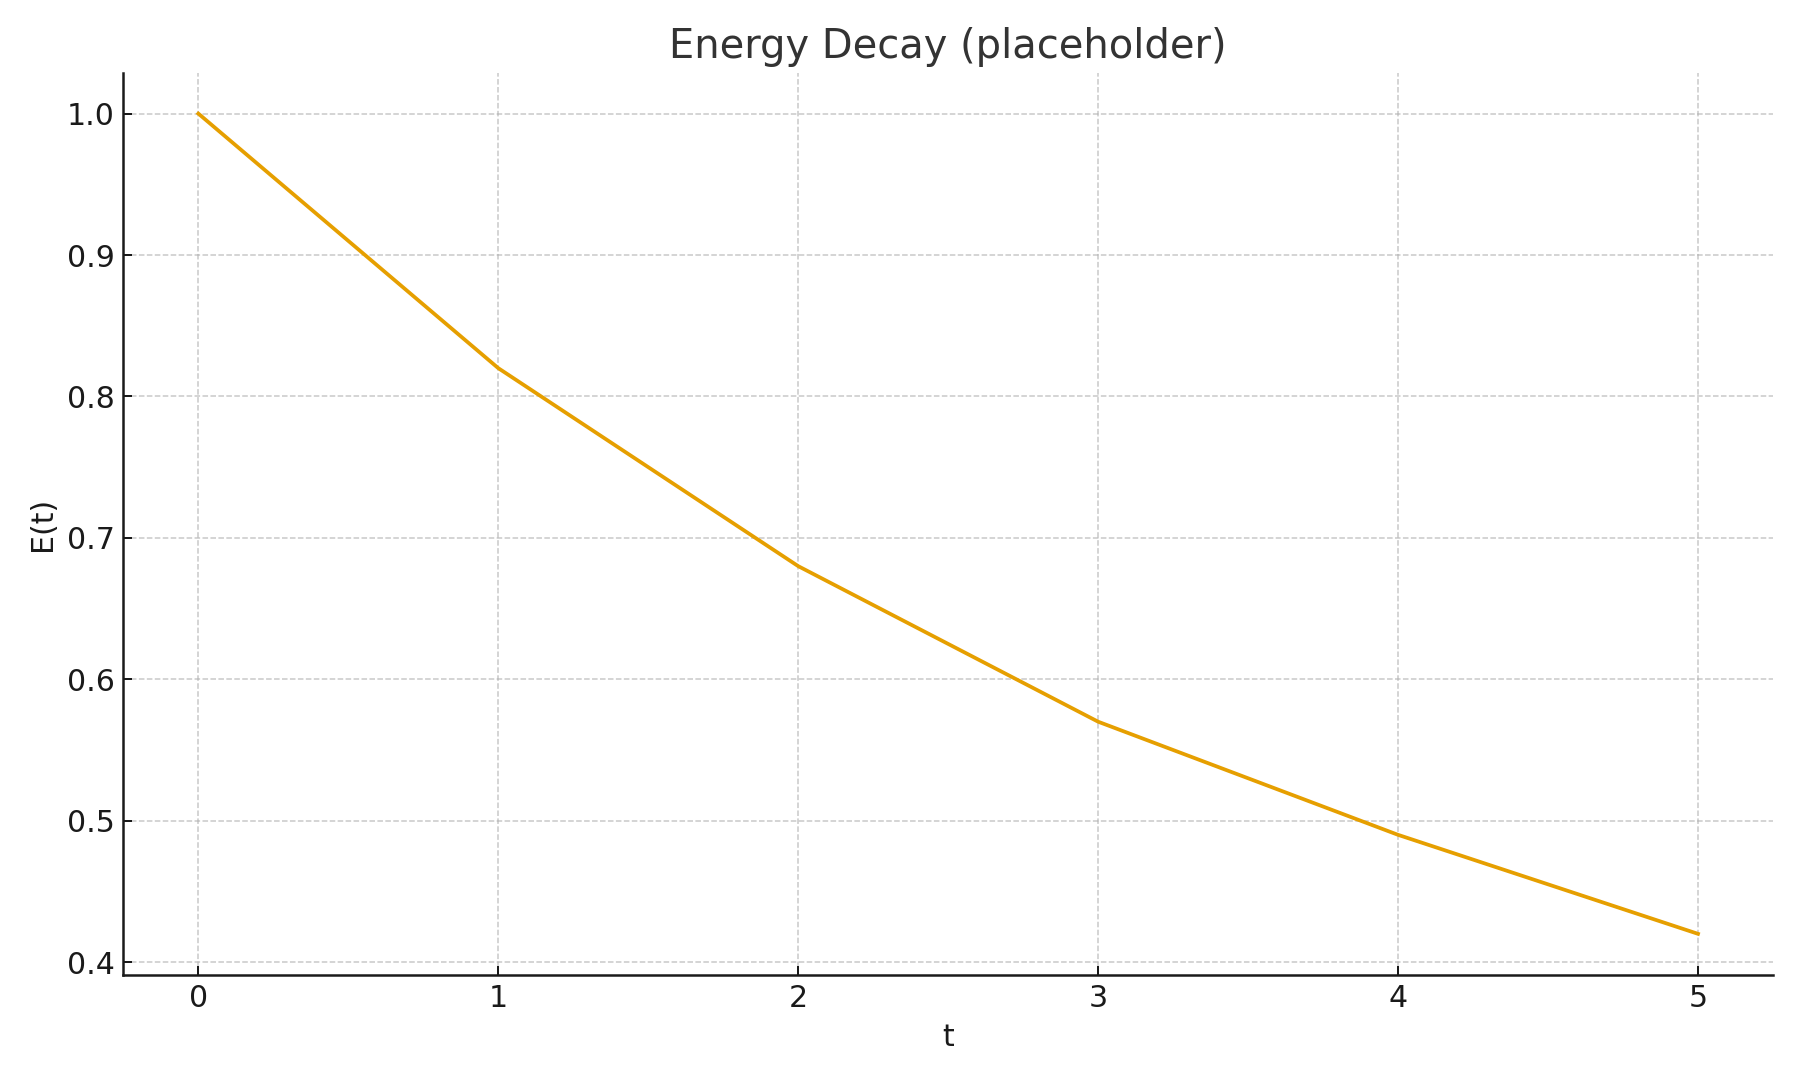
\includegraphics[width=.8\linewidth]{figures/energy_decay_placeholder.png}\caption{Energy trajectory (placeholder).}\end{figure}
\begin{figure}[t]\centering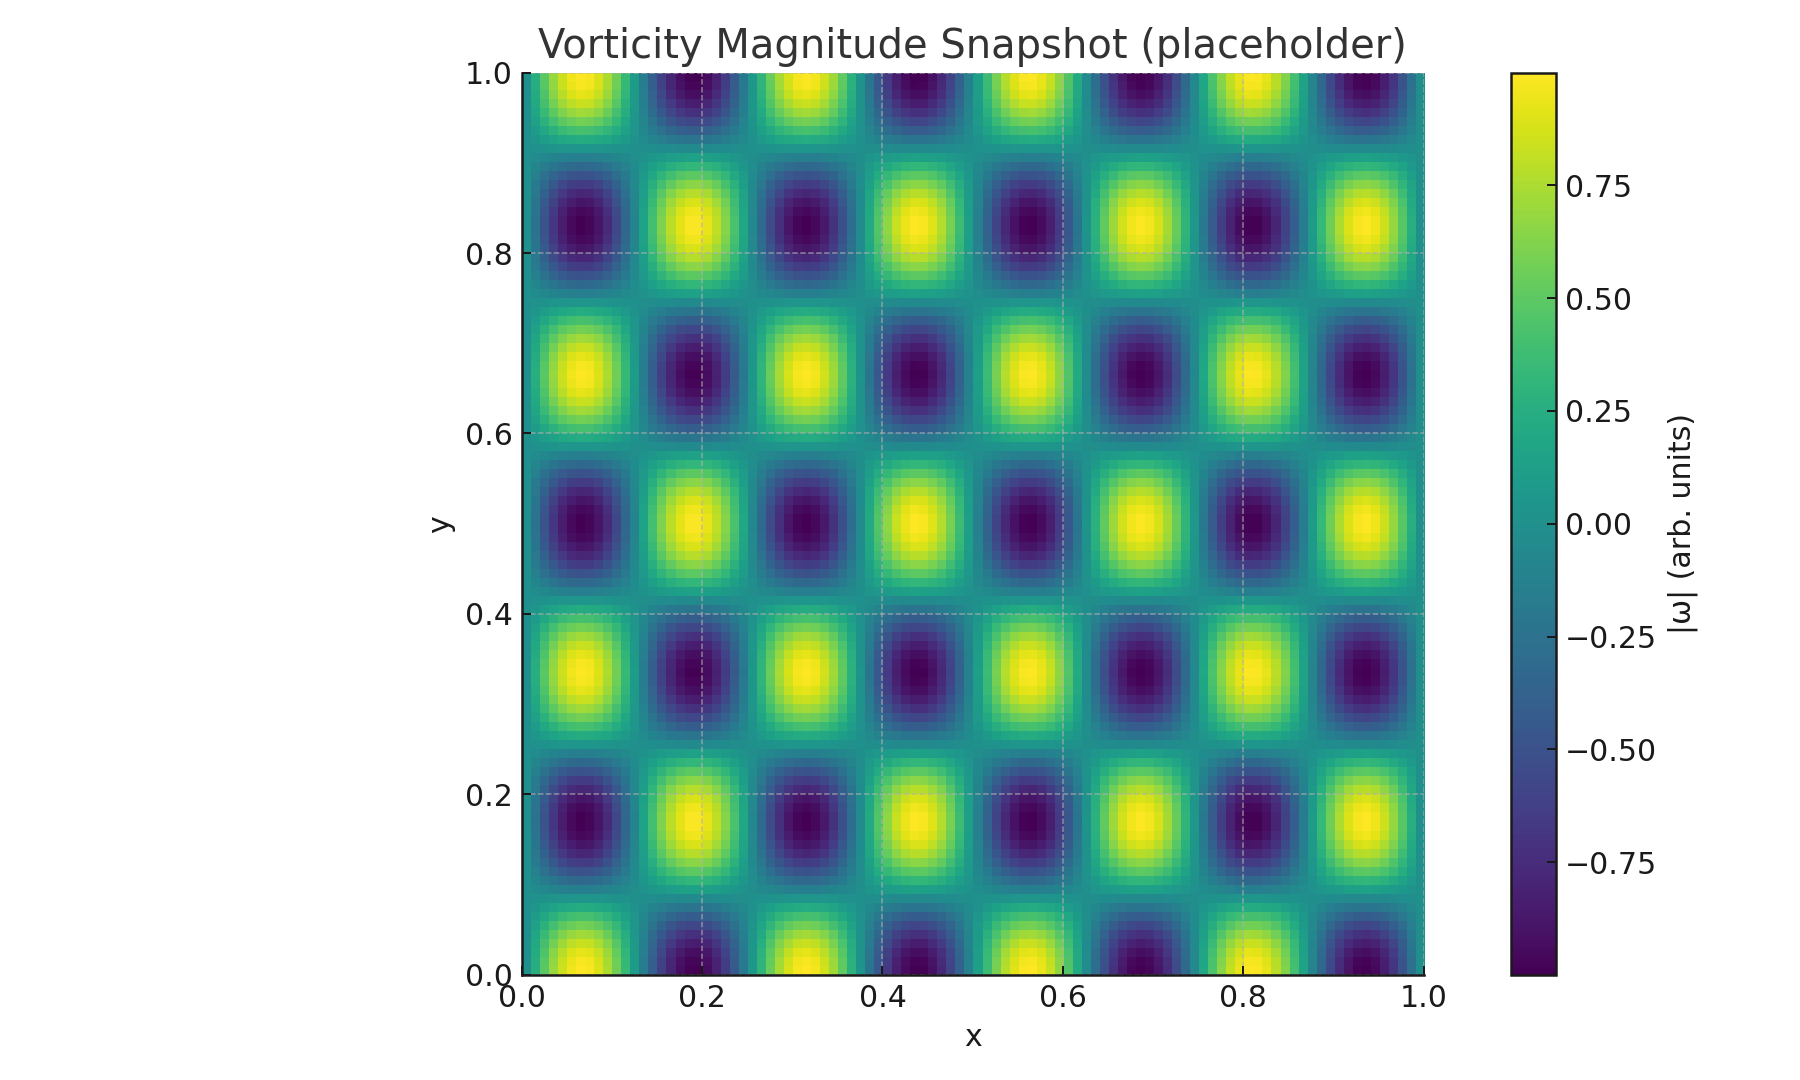
\includegraphics[width=.8\linewidth]{figures/vorticity_snapshot_placeholder.png}\caption{Vorticity magnitude snapshot (placeholder).}\end{figure}

\section{Discussion}
The ARP cascade rebalances dissipation across derivative levels while preserving viscous dominance; the remaining work is to pin down constants to close the master inequality.

\section{Scaling audit}
Navier--Stokes scaling: $u_\lambda=\lambda u(\lambda x,\lambda^2 t)$; $\omega_\lambda=\lambda^2\omega(\lambda x,\lambda^2 t)$.
ARP drives $\Phi_k=\|\nabla^k\omega\|_2^2$ strengthen with $k$, while $\lambda_k\alpha_k\propto 2^{-2k}$ keeps ARP's share subcritical relative to viscosity, preserving the criticality structure.

\section{Open problems}
Gap A: H$^1$ stretching constants; Gap B: high-order commutators; explicit schedule audit; critical scaling; link to Prodi--Serrin.

\section{Conclusion}
We reduced periodic global regularity to a concrete master inequality under an ARP-driven cascade and outlined the path to closing it.


\appendix
\clearpage

\section{Proof sketch of ARP barrier}
$\dot V = -(\nu-\lambda\alpha)\|\omega\|_2^2 - \lambda\mu G + \langle u,f\rangle$; with $f\equiv0$ and $\lambda\alpha<\nu$, strict decay follows.

\section{Commutator bounds}\label{app:comm}
Kato--Ponce/Moser templates: $\|\nabla^k(fg)\|_2 \lesssim \sum_{\ell=0}^k \|\nabla^\ell f\|_{p_\ell}\|\nabla^{k-\ell} g\|_{q_\ell}$, $1/p_\ell+1/q_\ell=1/2$.

\section{Gap A: H$^1$ vortex-stretching}\label{app:gapA}
$|\int (\omega\cdot\nabla)u \cdot \omega| \le \varepsilon_1 \|\nabla\omega\|_2^2 + C_\varepsilon \Omega^{3/2}$ via $\|\omega\|_{L^3}\le C \|\omega\|_2^{1/2}\|\nabla\omega\|_2^{1/2}$ and Riesz bounds.
Constant choices: with Riesz $C_R$ and GN $C_{GN}$, 
$|\int (\omega\cdot\nabla)u \cdot \omega| \le \varepsilon_1 \|\nabla\omega\|_2^2 + \frac{(C_R C_{GN}^3)^4}{4\varepsilon_1^3}\Omega^{3/2}$; take $\varepsilon_1=\tfrac12(\nu-\lambda_1\alpha_1)$.

\section{Gap B: high-order commutators}\label{app:gapB}
For $I_k=\int \nabla^k((\omega\cdot\nabla)u)\cdot \nabla^k\omega$, product/commutator splits and interpolation give
$|I_k|\le \varepsilon_k \|\nabla^{k+1}\omega\|_2^2 + C_\varepsilon \Xi_k(\{E_j\})$, with $\varepsilon_k=\tfrac12(\nu-\lambda_k\alpha_k)$.
Kato--Ponce/Moser constants $C_{KP}(k)$ and Riesz bounds $C_R(p)$ enter the polynomial $\Pi_k$ in the energies.

\section{GPU implementation details}
Spectral FFTs, semi-implicit viscous step, explicit nonlinearity, 2/3-rule de-aliasing, mild exponential filtering.

\section{Higher-order hierarchy}
Drive $G_k$ by $\|\nabla^k\omega\|_2^2$; augment $E_k$ with $\lambda_k G_k$ to tune dissipation across levels.

\section{Catalog of inequalities}\label{app:ineq}
Poincar\'e; Gagliardo--Nirenberg; Agmon; Riesz bounds $\|\nabla u\|_{L^p}\lesssim \|\omega\|_{L^p}$.

\section{Nondimensionalization}
In nondimensional variables with $Re=UL/\nu$, the constraint reads $\lambda'\alpha' < 1/Re$.

\section{Reproducibility checklist}
Commit hash; hardware; CUDA/FFT; grid and CFL; initial/forcing; $\nu$ or $Re$; controller $(\alpha,\mu,\lambda)$ and $(c_0,c_1,c_2)$; figure scripts.


\bibliographystyle{plainnat}
\bibliography{bib/references}

\end{document}
